% Chapter 1

\chapter{Contextual Enquiry} % Main chapter title

\label{contextualenqchapter} % For referencing the chapter elsewhere, use \ref{Chapter1} 

\lhead{Chapter \ref{contextualenqchapter}. \emph{Contextual Enquiry}} % This is for the header on each page - perhaps a shortened title

%----------------------------------------------------------------------------------------
\section{Study Description}
The purpose of this contextual enquiry was to elicit preliminary requirements to inform the design of an early prototype of a personal informatics application to be utilized through intermediaries. The study generated these requirements based on insights garnered from exploration of (1) issues related  to technology utilization; and (2) barriers to adoption of healthy behaviours. I was able to generate these insights from the data we collected in hospital settings with patients who qualify as prospective beneficiaries of such technology in future. The main goal of conducting a contextual enquiry was to gather contextual factors related to utilization of cellphone technology among obese adult patients. I obtained the ethical approval for this study from the Human Research Ethics Committee of the Faculty of Health Sciences at the University of Cape Town (see Appendix A).

I worked together with one research assistant in order to carry out this contextual enquiry. Between March 2013 and May 2013, we recruited a convenient sample of diabetic patients at the diabetes and endocrinology clinic at Groote Schuur Hospital in Cape Town. This is an outpatient clinic which runs on Thursdays and Fridays.

We opportunistically approached participants as they waited to see their doctors. We conducted interviews in one of the vacant consultation rooms, which guaranteed confidentiality and privacy of the participants. The main topics in these semi-structured interviews focused on participants' general utilization of mobile phones and specific usage for health, whether they sought help from intermediaries and, if so, who their preferred intermediaries were. In addition, we explored their current barriers to both exercise  and the adoption of a healthy diet.

We obtained our data from a total of 30 participants, 20 of whom were female. The majority of the participants had primary- and secondary-level education as shown in Figure \ref{figure:education_level}. The distribution of participants by ethnicity is shown in Table \ref{table:ethnicity} and all were from previously disadvantaged races during the apartheid era in South Africa. Most of the participants were low-income earners (Figure \ref{figure:income_distr}); this income data was for individuals and not households. Twenty-three percent had no income and depended on their family members to sustain them. In this group of people with no  sustainable income, only one person was 21 years of age, the remainder being above 40 years of age.
\begin{figure}[htbp]
  \centering
    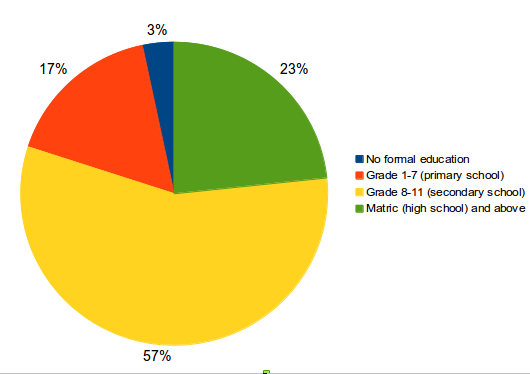
\includegraphics[width=0.6\textwidth]{Figures/education_level.png}
    \rule{35em}{0.5pt}
  \caption{Participants' education level.}
  \label{figure:education_level}
\end{figure}

\begin{table}[h!]
  \begin{center}
    \caption{Ethnicity of contextual enquiry's participants.}
    \label{table:ethnicity}
	\begin{tabular}{|p{3cm}|p{4cm}|p{2cm}|}
		\hline
		\textbf{Ethnicity}&\textbf{No. of Participants}&\textbf{Percentage}\\
		\hline
		 Black African&8 &26.67\% \\
		\hline
		 Coloured&22& 73.33\%\\
	\hline
	\end{tabular}
  \end{center}
\end{table}

\begin{figure}[htbp]
  \centering
    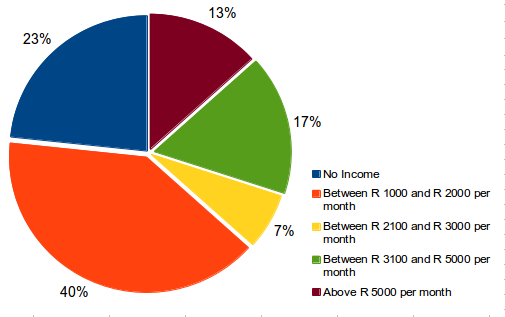
\includegraphics[width=0.6\textwidth]{Figures/income_distr.png}
    \rule{35em}{0.5pt}
  \caption{Participants' income distribution.}
  \label{figure:income_distr}
\end{figure}

Demographic information indicated the average BMI of the participants was reported to be 33.36 $kg/m^2$ (standard deviation of 5.74 $kg/m^2$); hence the majority of the participants were overweight, with fewer appearing to be clinically obese. The average age was 53.13 years old (standard deviation of 11.77 years old).  Almost 86\% (26) were above 40 years of age. This means we were dealing with old participants who were generally inexperienced or less conversant with technology.

\section{Data Collection Methods and Analysis}
We used a semi-structured questionnaire (Appendix E) to interview participants, each of whom was interviewed for 20 to 30 minutes. The questionnaire consisted of four groups of questions: demographics; cellphone ownership and utilization; access to information and pedometers; and barriers to diet and physical activity.~Based on their answers, we asked follow-up questions to seek clarifications on some of their responses.~We recorded responses for each participant on paper.

I used both descriptive statistics and qualitative approaches to analyse the information obtained from participants’ responses. Although our objective was to interview overweight and obese patients only, we included those who appeared to be thin but were diabetic. Since diabetes is a lifestyle-related disease, we felt that it would be interesting to also understand utilization of cellphones, and access to information even by individuals who appear not to be overweight but who may have some input in various issues related to technology utilization, and  barriers to adoption of healthy behaviours. All the names in the presentation of findings are pseudonyms to protect the privacy of participants. 
\section{Findings}
\subsection{Utilization of Cellphones}
Twenty-nine out of the 30 participants owned cellphones. The services most used were SMS and voice, with at least 80\% of the participants using both. At least 60\% of the phones owned by participants were smartphones (Figure \ref{figure:cell_ownership}), but utilization of functionality/services that are supported in smartphones was lower relative to voice and SMS (Figure \ref{figure:cell_utilization}). Utilization of services supported on smartphones only decreased with age. Utilization of WhatsApp was higher compared with other services that are specific to smartphones; participants were influenced to use WhatsApp by family members and friends who were already using WhatsApp. These influencers suggested that WhatsApp was cheaper than SMS. For instance, one 47-year-old male participant heard that WhatsApp was cheap for communication, and his son helped him load it on his phone. Therefore, in this context, social influence played a role in the adoption of some services that are supported only in smartphones. There is a positive correlation between social influence and adoption of high-tech innovations \citep{vannoy2010social}.  

\begin{figure}[htbp]
  \centering
    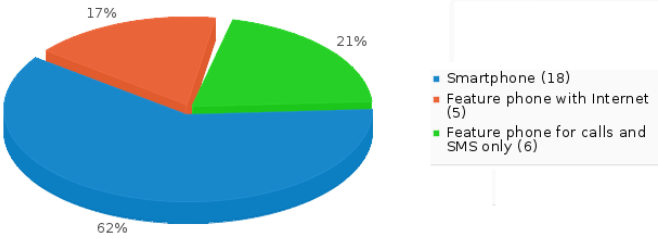
\includegraphics[width=0.5\textwidth]{Figures/cell_ownership.png}
    \rule{35em}{0.5pt}
  \caption{Participants' phone types.}
  \label{figure:cell_ownership}
\end{figure}

\begin{figure}[htbp]
  \centering
    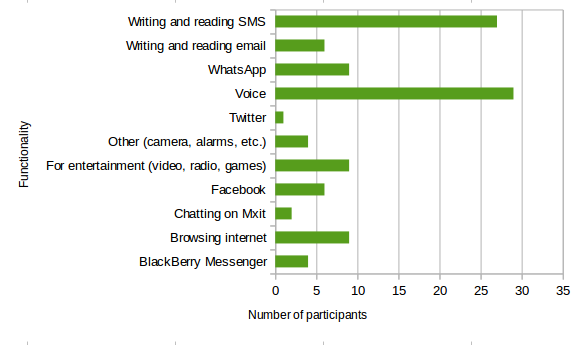
\includegraphics[width=0.5\textwidth]{Figures/cell_utilization.png}
    \rule{35em}{0.5pt}
  \caption{Utilization of cellphone functionality/services by participants.}
  \label{figure:cell_utilization}
\end{figure}
\subsection{Help-Seeking in Utilization of Cellphones}
There were several scenarios of informal help-seeking in utilization of cellphones as highlighted in Table \ref{table:intermediated}.

\begin{table}[h!]
  \begin{center}
    \caption{Scenarios of intermediated interactions.}
    \label{table:intermediated}
	\begin{tabular}{|p{0.5cm}|p{13cm}|}
		\hline
		 \textbf{No.}&\textbf{Scenario}\\
		\hline
		 1& Her \emph{daughter} helps her read SMSes by her, but she can do it on her own when the daughter is not around. \\
		\hline
		2&He doesn’t know how to reply to an SMS, so his \emph{grandson} always helps him with that.\\
	\hline
	  3&Her \emph{children} or  \emph{work colleagues} help her read SMSes written in English that are received through her feature phone. She also mentioned that her two children were more skilled than her in operating a cellphone one of them had a BlackBerry smartphone.\\
	  \hline
	  4&He can take photos using his mobile phone’s camera but he doesn't know how to save those photos on a memory card. His \emph{son} helps him with that once in a while. His son also helped him load WhatsApp on the phone.\\
	  \hline
	  5&Her \emph{children} have taught her how to use WhatsApp, take videos, etc. Now she is learning how to record sound and set alarm (reminders) on the phone for insulin and medication.\\
	 \hline
	 6&The \emph{son} helps her interact with the USSD service to check loyalty points on MTN. MTN is a mobile communication service provider operating in many African countries.\\
	 \hline
	7&She was taught by  her \emph{son} how to access a phonebook when composing SMSes using her new phone.\\
	\hline
	8&She receives assistance from her \emph{helper} when she wants to send messages to her children.\\
	\hline
	9&She was once helped to set up her new phone at a cellphone shop. She was also taught how to operate BBM by her \emph{grandson}.\\
	\hline
	10& He was once taught how to operate WhatsApp by his \emph{niece}.\\
	\hline
	11&Her \emph{son} and \emph{grandson} once helped to configure WhatsApp and Facebook on her phone. They have also taught her how to use those two web services. In addition, she also asks the son to search for certain health information on the Internet, and once the search is done the son passes the phone to her to view that information. This happens once a month.\\
	\hline
	12& Her \emph{son} and \emph{grandson} teach her how to use various functionalities like games, etc., but she is not that keen on operating those functionalities. She also admitted that her son and grandson are very interested in their mobile phones and they spend a lot of time playing on their phones, which is something she doesn't understand.\\
	\hline
	13& This participant does not own a cellphone. She has no formal education and is unfamiliar with how to operate a cellphone. Her son receives SMSes directed to her and reads them aloud for her or translates an SMS to verbal communication. Also, the son receives phone calls and hands over the phone to her when the person on the other end of the line wants to speak to her.\\
	\hline
	\end{tabular}
  \end{center}
\end{table}

The majority of the participants had solicited  informal help from other people before to configure services/apps on their phones (e.g. WhatsApp, Facebook); in the habituation of skills required for utilization of various functionalities (e.g. a phonebook of a new or unfamiliar cellphone, WhatsApp); and to interact with certain features such as SMS and Internet browsers.

There was a variation in the degree of help-seeking that was determined by how often participants wanted to execute unfamiliar tasks. Tasks such as configuration of services and apps or teaching of individuals were rare occurrences, as they only happened when participants encountered a new application or device and did not know how to make it functional. For frequent used applications, where participants were not able to utilize them entirely on their own, they sought for assistance by intermediaries more often. The next section highlights the characteristics of intermediaries that were mostly picked by participants.
\subsection{Selection of Help-Givers}
Participants chose trusted individuals to act as their help-givers, typically their children and grandchildren or, less often, children of relatives, family friends, or someone at a cellphone shop. The most likely to be solicited to assist were family members. Help-givers were selected based on the merit of skills/competence; interpersonal trust based on a social relationship; and past experience of help-seekers with specific help-givers.
\subsubsection*{Interpersonal trust}
Interpersonal trust in this context means whether help-seekers feel comfortable seeking help from specific people or not. Privacy and the existing relationship between a help-seeker and help-giver were the first concerns when deciding who to ask for help. An additional factor was whether the help-seeker could trust a helper-giver to deliver when solicited for help and this was influenced by past attempts -- positive and negative -- at seeking help. These experiences shaped perceptions of some of the participants about seeking help with cellphone or any other technology. For instance, one  67-year-old female participant reported that her daughter helped her once but she had no patience. A male participant aged 47 mentioned that he would like assistance when using services such as MMS, but that young people do not have patience to help. Such negative experiences can prevent help-seekers asking certain help givers for assistance. This resonates with the finding by~\cite{kiesler:twi} that parents may be reluctant to seek informal help from their children after encountering negative experiences.
\subsubsection*{Help-givers' Competence}
In addition to interpersonal trust, deciding who to solicit for help was also influenced by the help-seekers' level of trust of the skills possessed by help-givers. Participants were confident that their children could use cellphones competently. Several participants thought their children had the technical know-how to use cellphones. For instance, one 31-year-old female participant mentioned that her five-year-old son knows how to navigate through her entire phone and use it more than she does. Another female participant, aged 56, explained how children are eager to teach her various things on a cellphone but she is not that keen to use cellphones like her son and grandson do. A 47-year-old male participant, mentioned that, within the family, young people are more skilled at using cellphones than old people.
Participants reported that their kids were borrowing their phones to do other tasks and this demonstrated that their kids had better skills with technology. Scenarios of sharing are presented in Table \ref{table:phone_sharing_contextual} below. 

\begin{table}[h!]
\begin{center}
    \caption{Scenarios of sharing of cellphones between participants and their children.}
    \label{table:phone_sharing_contextual}
	\begin{tabular}{|p{1cm}|p{12cm}|}
		\hline
		 \textbf{No.}&\textbf{Scenario}\\
	\hline
	1&``Zandile'', a 47-year-old female, mentioned that her 16-year-old son would borrow her phone to use Mxit. Zandile does not use anything else on the phone apart from calls and SMS. She also said that she is not much interested with technology. For example, she has Internet at work, but does not really use it.\\
	\hline
  2& ``Buyisiwe'', a 31-year-old female, narrated an experience about her five-year-old son who uses her smartphone to listen to music. But she has to lock it while he is listening, because on one occasion he deleted almost everything on the phone.\\
  \hline 
  3&``Celine'', a 48-years-old female, lends her phone to her daughter who uses it for normal Internet browsing and Facebook. Celine owns an advanced feature phone that is Internet-enabled, but she does not use Internet on the phone.\\
  \hline
	\end{tabular}
  \end{center}
\end{table}
In other scenarios, participants mentioned that their kids borrow their phones to search for information related to school assignments. These examples demonstrate the level of skills that potential help-givers can have. Trust in the skills possessed by help-givers has been found to be very important to individuals seeking help in the ICTD and HCI contexts.~\cite{ramirez2013infomediaries} suggests that empathy and technical skills of infomediaries influence the outcomes of the process of infomediation to users at public access venues. Another study that examined motivations for informal support in utilization of computers at home found skills of help-givers to be one of the factors that influence help-seekers to solicit help from specific people~\citep{poole:chh}. 
\subsection{Access to Health Information and Self-Monitoring Support}
We also collected data on how participants currently access information pertaining to health. In addition we collected data on how participants' currently self-monitor health. Informational support on which most of the participants rely is that provided through face-to-face meetings with doctors or dietitians during hospital visits. Normal hospital visits are scheduled every three or six months, but participants visit the hospital only two or three times a year. In addition to face-to-face information, patients normally receive paper sheets that provide guidance on how to eat healthily. These are usually received when patients attend the clinic for the first time after being diagnosed with diabetes. Most patients we interviewed were type 2 diabetics and overweight. Doctors and nurses encourage them to eat healthily and to exercise. 

The majority of the participants lacked informational support beyond hospital settings that could provide guidance for healthy eating  and exercising.~Very few participants had used cellphone services to query or receive information related to health. Only six participants had used the Internet to search for health information, while only one participant had used a cellphone app for health. Only two participants had used SMS, while only one had used voice to look for health information. Table \ref{table:health_information} shows some of the scenarios of were participants used ICTs in relation to learning about issues concerning their health.
\begin{table}[h!]
\begin{center}
    \caption{Participants’ usage of ICT to fulfil health information needs.}
    \label{table:health_information}
	\begin{tabular}{|p{1cm}|p{12cm}|}
		\hline
		 \textbf{No.}&\textbf{Scenario}\\
		 \hline
		 1&``Anitha'', a female participant aged 56, sends SMSes to her son while he is at his workplace. These are usually requests to check for certain  health information on the Internet, and the son then prints all the relevant material. She also follows Dr Oz's program on TV about health issues. If she misses an episode, she goes onto the Internet and visits the programme's website\\
	  \hline
	  2& ``Jane'', a female participant aged 36, has an app on her phone for giving health tips. She downloaded the app from the Internet.\\
	  \hline
	  3& ``Maria'', a female participant aged 57, mentioned that she uses Facebook.~She has three diabetic friends and they share diet concerns, recipes, and discuss diabetic-specific issues that they experience. They do not discuss exercise. She sometimes searches on Google for medication, especially when she starts using new medications. She uses Google to get more information on the things her doctor advises.\\
	  \hline
	  4& ``Evelyn'', a female participant aged 63, subscribes to health websites to receive emails with health tips and information. She sometimes calls a dietitian to ask about certain diet information.\\
	  \hline
	\end{tabular}
  \end{center}
\end{table}

Self-monitoring of blood glucose was common among the participants, because many of them were diabetic. There was less frequent self-monitoring of other health parameters such as diet and physical activity by many participants. Of the 30 participants we interviewed, only two participants had used a pedometer before.  One participant had used a gym bicycle with a meter that shows distance cycled but she stopped using it. Only eight participants reported that they had used a diary before to record the food they had eaten. But this was not consistent. Some stopped doing it, although they claimed that when they visit hospital, the sisters (nurses) always remind them to record foods they have eaten, which is mainly for controlling the levels of blood glucose. For instance, one participant said that she records both what she has eaten and the blood glucose levels before and after meals. Overweight and obese diabetic patients are also encouraged to lose weight, because losing weight has an advantage of lowering levels of blood glucose.  The recommended approach for weight loss is to follow the recommended diet and become more physically active. 
\subsection{Barriers to Adoption of Healthy Behaviours.}
The research teams also examined barriers to adoption of healthy behaviours, such as a healthy diet and exercise.

In this regard, 76\% of the participants said that the recommended healthy food is always expensive. For instance, fat-free foods are much more expensive than full-fat foods. One participant associated the eating of certain food with cultural upbringing. She explained that Muslims in Cape Town often have very high fat and high sugar content foods  such as samosas. One of the comments that many participants made was that it is difficult to have a budget for separate meals within the family, because diabetic members always have their diet food which is not popular with the rest of the family. So, diabetic members might end up eating what the rest of the family eats. They do try to have diet foods, but it is not always manageable. One participant who seemed to be highly motivated disagreed with that argument and said most people lack an understanding of what carbohydrate means. She further mentioned that education about diet should be contextualized to terms that people are already familiar with. She said most people don't understand what is said by dietitians because it is not communicated in the context they understand. For example, the concept of carbohydrates is not well comprehended by many people, but if the topic is well explained using what is already familiar to patients, then they are more likely to understand.

On the question of perceived barriers to physical activity, nine participants mentioned that lack of time to do physical activity because of a busy schedule contributes to less exercising. This is supported by some remarks shared by participants in Table \ref{table:busy_schedules}. 

\begin{table}[h!]
\begin{center}
    \caption{Excerpts of participants’ common remarks on the association between being less active and busy schedules.}
    \label{table:busy_schedules}
	\begin{tabular}{|p{2.5cm}|p{10.5cm}|}
		\hline
		 \textbf{Participants}&\textbf{Remarks}\\
	  \hline
	  1&She goes to work very early in the morning and comes back late at night.\\
	  \hline
	  2&Difficult to manage work and household.\\
	  \hline
	  3&She goes to work at 4.00 am and comes back at 7.00 pm. She works six days a week.\\
	  \hline
	  4&She looks after the family. She takes her sister's child to school and does the cooking. She does a lot of housework. So it is difficult to have a planned series of physical activity.\\
	  \hline
	 5&Difficult to find balance between planned session for physical activity and manage both work and household at the same time.\\
	 \hline
	 6&Busy with housework at home.\\
	 \hline
	\end{tabular}
  \end{center}
\end{table}

Seven participants said that the lack of areas to walk around is one of the barriers to physical activity. The most common comment in support of this argument was that most of the areas where they live are not safe for somebody to be out walking all the time (Table \ref{table:safety_issues}). Most of these areas have high rates of crime.

\begin{table}[h!]
\begin{center}
    \caption{Excerpts of participants’ remarks on safety concerns about areas to walk or run.}
    \label{table:safety_issues}
	\begin{tabular}{|p{2.5cm}|p{10.5cm}|}
		\hline
		 \textbf{Participants}&\textbf{Remarks}\\
	  \hline
	  1&The neighbourhood is not safe to wander around.\\
	  \hline
	  2&It is not safe in her area. She doesn't like to be outside most of the time.\\
	  \hline
	  3&It is unsafe at night and early morning.\\
	  \hline
	  4&The area where she stays is not safe to walk around.\\
	  \hline
	 5&Not safe to walk alone. She prefers to walk through houses.\\
	 \hline
	\end{tabular}
  \end{center}
\end{table}

But despite the lack of both time and areas to exercise, these participants mentioned that they are active when doing their daily errands (Table \ref{table:daily_activity}). 

\begin{table}[h!]
\begin{center}
    \caption{Excerpts of participants' remarks regarding physical activities that were part of their daily routines.}
    \label{table:daily_activity}
	\begin{tabular}{|p{2.5cm}|p{10.5cm}|}
		\hline
		 \textbf{Participants}&\textbf{Remarks}\\
	  \hline
	  1& She walks from home to visit relatives and friends.\\
	  \hline
	  2&He only walks when he goes to church.\\
	  \hline
	  3&She walks from her home to a bus station every day and walks a lot at work, so it would be great for her to have something to keep track of how much exercise she gets. She wants to be more active but works seven days a week.\\
	  \hline
	  4&She exercises in a group of people three times a week and now feels much healthier. They have a ``biggest loser'' competition going at the moment. She would like to have a pedometer to keep better track of her activity.\\
	  \hline
	 5&She walks only when she has to. She only walks up and down in the kitchen. She has a treadmill, but she doesn't use it.\\
	 \hline
	\end{tabular}
  \end{center}
\end{table}

\section{Contextual Design Insights}
These are some of the design insights that were uncovered from the aforementioned findings. In this context, the majority of the participants did not utilize ICTs in self-management of their health, as they relied only on paper diaries. The only parameter that was being monitored by the majority of the participants was blood glucose, as all participants were diabetic. Blood glucose is usually controlled through factors such as diet, exercise and medication. Type 2 diabetes is linked to obesity and its self-management is mostly through diet and exercise.  The process of self-management can be very cumbersome if it is done using pen and paper and this may reduce compliance \citep{mattila2008mobile}. A paper diary may not be as effective as an electronic diary when it comes to navigating behaviour patterns for the purpose of self-reflection. Therefore, personal health apps may be important in supporting self-management of health. However, these apps might not be very useful in this context considering the fact that most of the participants have limited skills in operating technology. The findings above indicate that some participants with limited skills seek help from people with skills. But this approach has its limitations, as it relies on existing intrinsic motivation of help-givers. Long-term usage is crucial for compliance~\citep{mattila2008mobile}, but one cannot achieve this long-term usage in the context where a technology needs to be utilized through help-givers, while most technologies were not designed to anticipate utilization through help givers as part of the usage ecosystem. As it has been advocated, novel approaches such as ICTs in lifestyle modifications may facilitate moving the management of lifestyle-related chronic conditions from healthcare systems to citizen-centric health promotion and disease prevention interventions~\citep{korhonen2010personal}; hence it is important for one to think of how to design technologies that can scale to demographics that are not well considered in traditional interface design. Intermediated technology use  is one of the interaction models that we need to consider.

Findings above demonstrate scenarios of intermediated technology use, that may be common in contexts with technology users with similar characteristics as our participants. For instance, a participant in Table \ref{table:intermediated} (No. 11), puts requests to her son to search for certain health information on the Internet and the son passes the phone back to her. In this case, the beneficiary user has an intent that is translated into actions on a technology by the intermediary user. If we refer to literature review (Chapter \ref{literaturereview}), ~\cite{sambasivan2010} has described this type of intermediation as ``proximate-enabled translations of intents to input into technology''.  

I made several decisions that were crucial to the design of the first prototype.  Since participants reported to have activities related to NEAT (non-exercise activity thermogenesis) in their daily life, the first decision was based on the idea to promote NEAT since it has proved to be beneficial in improving well-being. The second consideration was about  promoting healthy eating habits using a metaphor that was already used by dietitians. In order to educate patients, dietitians used a meal chart to reflect what a plate of healthy food looks like. The third design decision was how to design motivational affordance to promote collaboration between help-seekers and help-givers. This was inspired by the finding about sharing phones between adults and kids, namely that kids borrow phones from their parents because they are motivated by specific things on the phone. Some of those are social media, games and music. Therefore, if one could design a system with specific motivational affordances that address the needs of kids and then integrate those affordances with self-monitoring of adult behaviours, then it is possible to enhance the motivation of kids to help their parents with self-monitoring tasks. With the guidance of self-determination theory, and techniques that have been used in the previous studies that utilized gamification (described in the \emph{Literature Review} chapter), I developed the first prototype. The iterations of prototype development and subsequent evaluations are discussed in the following chapters.

\begin{flushright}
\end{flushright}